\documentclass{llncs}

\usepackage[utf8]{inputenc}
\usepackage[english]{babel}

\usepackage{amsmath,amsfonts,amssymb}
\usepackage{array}
\usepackage{url}

\usepackage{tikz,pgfplots}

\tikzset{
  baseline=(current bounding box.center)
}

\newcommand{\doctype}{Parallel Radix Sort on OpenCL}

\usepackage{hyperref}
\hypersetup{
  breaklinks=true,
  colorlinks=true,
  citecolor=blue,
  linkcolor=blue,
  urlcolor=blue,
  bookmarksnumbered,
  bookmarksopen,
  pdftitle={\doctype},
  pdfauthor={Hennadiy Yatskov, Nico Mürdter},
  pdfsubject={},
  pdfkeywords={},
}

% Final Submit TODO: remove following line which makes margins smaller
\hypersetup{pdfpagescrop={92 62 523 748}}

\usepackage{breakurl}

\title{\doctype}
\author{Hennadiy Yatskov\\ Nico Mürdter}
\institute{
Karlsruhe Institute of Technology, Karlsruhe, Germany\\
\email{hennadiy.yatskov@student.kit.edu\\ nico.muerdter@student.kit.edu}}

\begin{document}

%% sp-process: load data in sql-table 'stats'
% IMPORT-DATA stats ../run.log

%% DEFMACRO REFORMAT(precision=0)
%% SELECT MAX(it) AS iterationcnt FROM stats
\def\iterationcnt{5}

\maketitle

\begin{abstract}
TODO
\end{abstract}

% Final Submit TODO: remove this prior to FINAL submission
\pagestyle{plain}

\section{Algorithm}
\label{Algorithm}
This algorithm is based on an open source implementation of P. Helluy \cite{ocl-radix-helluy}. Before we come to the detailed explanation of the algorithm, we first need to define several values. $K(j)$, represents the non-sorted input values which consist only of integers. The implementation of P. Helluy is only capable of sorting 32-bit unsigned integers. So in his implementation, each of these integers in $K(j)$ for $j=0 \dots N-1$ is positive and will be called a \textit{key} in the further explanation. To expand the usage of this algorithm, this draft explains the expansion to support also 64-bit unsigned integers, and signed 32 and 64-bit integers. Because of the fact, that Radix-Sort is a non-comparative integer sorting algorithm, this implementation will not support floating point numbers. In order to allow operation with signed integers, an offset is added to the integers. This offset is in case of a signed input list, the absolute value of the minimum possible value of the given integer. In case of a 32-bit signed integer this would be $abs(-2^{31})$. The GPU kernels are still working on the unsigned representation of the given input data type, and the offset incrementation is done on the fly, when the key is first accessed. Also the decrementation at the end of the algorithm is done on the fly to prevent performance losses. So basically from the outside it seems the algorithm is working directly on the signed integer values, but on the inside it is working with a shifted number range to fit into the unsigned number range.

The Radix is represented by $R = 2^r$ where $r$ is the number of bits necessary representing $R$. We suppose that $b$, the total number of bits representing the keys is divisible by $r$ and so the number of passes is denoted by $p = b/r$. This assumption can be satisfied by an appropriate definition of $r$. Each pass $q=0 \dots p-1$ of the algorithm consists in sorting the list according to the $q^{th}$ digit (in base $R$) $K(j)_q$. A pass can be imagined as a reordering of the list by this $q^{th}$ Radix. So after $p = b/r$ passes the list is sorted totally. It is important to say, that each pass sorts the corresponding elements in a stable manner. So the work done in each pass is not corrupted by previous passes and will not corrupt following passes.

The final algorithm is seperated into three different phases, which are executed consecutively in every pass. These phases are called Histograming, Scanning and Reordering. The explanation is listed below.

%If the number of elements in $K$ can't satisfy this assertion, it will be extended with maximum integer values so that is satisfies it. This extension is done with maximum values, so that the sorting is only influenced in the first phase of the algorithm, which will be explained in the next sections.


\subsection{Histograming}
This first phase of the algorithm is in charge of calculating key \textit{histograms}. A histogram represents the number of occuring Radix in the given list of elements $K$. To do this fully parallel, the porcessing units are seperated in Groups $G$ with Items $I$, where an Item represents a Processor. So based on the GPU Architecture, the total amount of available Processing Units is $GI$. For the explanation we can suppose, that $N=GI$. If this is (most likely) not the case in a real scenario, the data is extended by adding keys which represent the biggest possible value. Each Item is in charge of a part of the list. It computes the Histogram of its own sublist and adds his histogram to the histogram of the Group. This is simply done by just inspecting every element in the list, computing every $q^{th}$ bit sequence with the length $r$ and then incrementing the corresponding entry in the local Histogram, which represents the computed Radix.

%TODO Geschickte Groupwahl etc noch einbringen.

\subsection{Scanning}
The next step in this algorithm is the so called Scanning. In this part the calculated Histograms are collected over a Prefixsum algorithm. P. Helluy \cite{ocl-radix-helluy} and also the here shown improved implementation is using the Blelloch algorithm for parallel scans \cite{blelloch1989scans}. After the Prefixsum, every Processor knows in his own Histogram, how many elements according to the current Radix are smaller. This information given by the Prefixsum, allows a reordering based on the calculated Histograms from the previous section.

\subsection{Reordering}
To finally reorder the elements, the Prefixsum of the Histograms is needed. As described in \cite{ocl-radix-helluy}: \textit{after the prefix sum, the histogram $H(c, g, i)$ contains the position, in the ordered list, of the first key with radix $c$ that is examined by the item $i$ in the group $g$.} So the Histogram can than be used to reorder the elements acording to the Radix of the corresponding pass. To do this reordering, every Processor once again looks at the Radix of the current pass of every element, and then moves the element to the new position according to the Histogram. Afterwards the entry in the Historgam is increased by 1 for the next element with the same Radix. This reordering can also be done fully parallel.

\newpage
\section{Implementation Details}
In this chapter the focus lays on the implementation. The basecode is written for OpenCL 1.2. The main routine focuses on instantiating buffers and delegating the computational tasks to the GPU processors. The three main parts, shown in \ref{Algorithm}, are represented by so called OpenCL kernels. For each of these described tasks one kernel is in charge. Because a GPU is a PRAM architecture, all processors are working on the same main memory. So the main difficulty here was to effectively seperate the memory each Processor is working on to avoid data corruption. To achieve this the kernels made use of the standard OpenCL routines to get to know what their operating ranges are on the main memory. This restriction also allows to use the OpenCL \textit{restrict} keyword, which gives the compiler a hint, that the marked buffers' adress spaces do not overlap. Therefore, the compiler is able to increase the overall performance by making use of cache optimizations.

To ensure the usage of different datatypes on the same codebase, this implementation is heavily based on the concept of C++ templates. The whole sorting algorithm can be instantiated with one of 4 supported data types: int32 / int64 / uint32 / uint64. This makes it easy to use this implementation for further projects without the need to accept performance losses if only 32-bit integers are of interest.

These type restrictions can easily be handled in C++ but for OpenCL we needed a more special method. Usually, the codebase of the OpenCL kernels is loaded during runtime and then compiled for the local GPU. Right before the compilation the code is imported with appended prepocessor \#define directives which set the internal data types to either 32 or 64 bit unsigned integer and the \textit{offset} show in \ref{Algorithm} to the appropriate value, which depends on whether the input data type is signed or unsigned.

Another notable implementation detail is the usage of local memory and barriers within the OpenCL code. The processors need to be aligned after several operations like copying the histograms to the local memory. To avoid data corruption these actions are controlled by memory barriers. The usage of the local memory of every processor leads once again to an overall significant performance increase as it allows for a considerable boost in access time and can be, broadly speaking, regarded as a cache.
% \subsection{Kernel}

\newpage
\section{Experimental Results}
All experimental benchmarks were made on a NVIDIA GeForce GTX 680 and a Intel i7-3770K CPU. GPU Driver Version 361.91 with OpenCL 1.2. For comparison the data was also sorted with std::sort and a custom single threaded Radix-Sort implementation on the CPU. The test data consisted of 5 different datasets:

\begin{enumerate}
  \item \textbf{Zeros}\\ Dataset containing only zeros
  \item[]
  \item \textbf{Random}\\ Dataset containing random generated integers by a mersenne twister
  \item[]
  \item \textbf{RandomDistributed}\\  Dataset containing random generated integers by a uniform distribution random generator
  \item[]
  \item \textbf{Range}\\ Dataset containing a sorted range of integers beginning by the minimum value of the used datatype
  \item[]
  \item \textbf{InvertedRange}\\ Dataset containing the integers from range in inverted order
\end{enumerate}

% Your hardware.

% What do you benchmark.

% Running time~\ref{fi:runningtime:uniform} and speedup plots~\ref{fi:speedup:uniform} (for each generator, 64-bit integer and 32-bit floating point (not for  non-comparative integer sorting algorithms).

% Interpretation.

\begin{figure}[h!]
\centering
\pgfplotsset{compat=1.5}
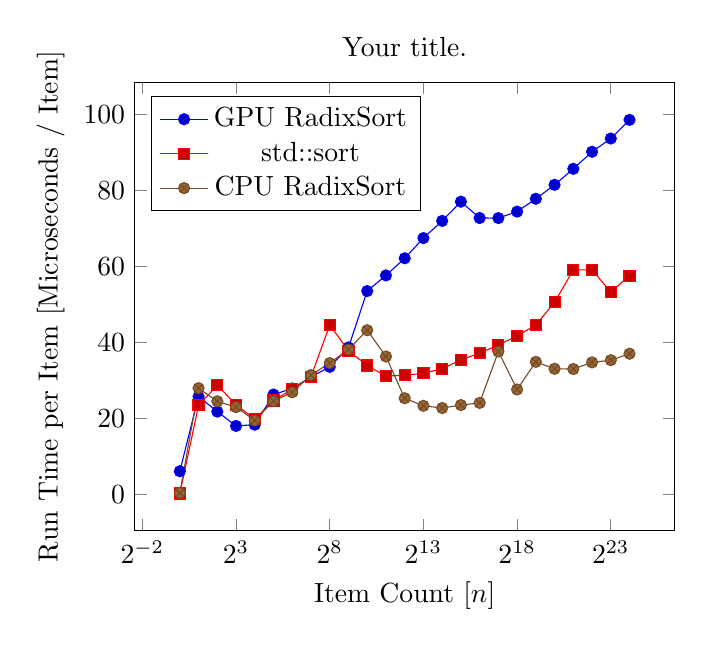
\begin{tikzpicture}[scale=1]
  \begin{axis}[
    title={Your title.},
    xlabel={Item Count [$n$]},
    ylabel={Run Time per Item [Microseconds / Item]},
    legend pos=north west,
    xmode=log,
    log basis x={2},
    ] 
    %% MULTIPLOT(threads) SELECT n AS x, (avg("wall-time") * 1.0 / n) AS y, MULTIPLOT
    %% FROM stats
    %% WHERE it > 0 AND "input-type"='uniform'
    %% GROUP BY MULTIPLOT,x ORDER BY MULTIPLOT,x
    \addplot coordinates { (1,6.14588) (2,25.8) (4,21.85) (8,18.075) (16,18.4125) (32,26.3438) (64,27.9469) (128,30.9563) (256,33.6352) (512,38.7367) (1024,53.5891) (2048,57.7013) (4096,62.2103) (8192,67.5351) (16384,72.0565) (32768,77.1085) (65536,72.8129) (131072,72.7906) (262144,74.5003) (524288,77.8793) (1048576,81.5511) (2097152,85.7657) (4194304,90.2553) (8388608,93.7425) (16777216,98.6555) };
    \addlegendentry{GPU RadixSort};
    \addplot coordinates { (1,0.2998) (2,23.5) (4,28.8) (8,23.675) (16,19.85) (32,24.75) (64,27.7625) (128,31.0453) (256,44.6383) (512,37.8852) (1024,33.967) (2048,31.1891) (4096,31.4354) (8192,31.9057) (16384,33.1395) (32768,35.4618) (65536,37.2686) (131072,39.349) (262144,41.8065) (524288,44.6163) (1048576,50.6581) (2097152,59.1302) (4194304,59.1624) (8388608,53.3066) (16777216,57.644) };
    \addlegendentry{std::sort};
    \addplot coordinates { (1,0.4005) (2,28) (4,24.55) (8,23.025) (16,19.525) (32,24.5875) (64,26.925) (128,31.4609) (256,34.6203) (512,38.2023) (1024,43.274) (2048,36.3531) (4096,25.3622) (8192,23.3748) (16384,22.7897) (32768,23.568) (65536,24.1379) (131072,37.6677) (262144,27.6724) (524288,34.9413) (1048576,33.1177) (2097152,33.0524) (4194304,34.8011) (8388608,35.3875) (16777216,37.0874) };
    \addlegendentry{CPU RadixSort};
  \end{axis}
\end{tikzpicture}
\caption{Runtimes of \texttt{std::sort} with uniform input. Mean of \iterationcnt~iterations.}
\label{fi:runningtime:uniform}
\end{figure}

\begin{figure}[h!]
\centering
\pgfplotsset{compat=1.5}
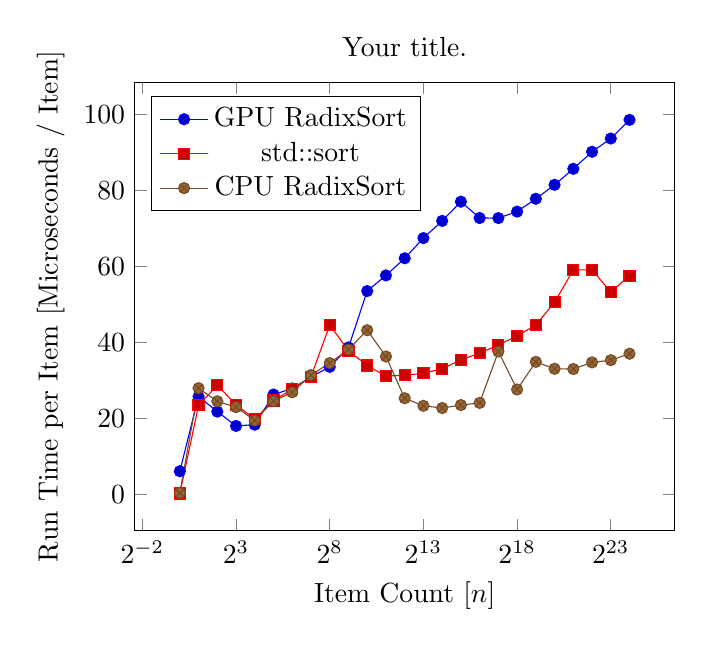
\begin{tikzpicture}[scale=1]
  \begin{axis}[
    title={Your title.},
    xlabel={Item Count [$n$]},
    ylabel={Run Time per Item [Microseconds / Item]},
    legend pos=north west,
    xmode=log,
    log basis x={2},
    ] 
    %% MULTIPLOT(threads) SELECT n AS x, (avg("wall-time") * 1.0 / n) AS y, MULTIPLOT
    %% FROM stats
    %% WHERE it > 0 AND "input-type"='uniform'
    %% GROUP BY MULTIPLOT,x ORDER BY MULTIPLOT,x
   \addplot coordinates { (1,6.14588) (2,25.8) (4,21.85) (8,18.075) (16,18.4125) (32,26.3438) (64,27.9469) (128,30.9563) (256,33.6352) (512,38.7367) (1024,53.5891) (2048,57.7013) (4096,62.2103) (8192,67.5351) (16384,72.0565) (32768,77.1085) (65536,72.8129) (131072,72.7906) (262144,74.5003) (524288,77.8793) (1048576,81.5511) (2097152,85.7657) (4194304,90.2553) (8388608,93.7425) (16777216,98.6555) };
    \addlegendentry{GPU RadixSort};
    \addplot coordinates { (1,0.2998) (2,23.5) (4,28.8) (8,23.675) (16,19.85) (32,24.75) (64,27.7625) (128,31.0453) (256,44.6383) (512,37.8852) (1024,33.967) (2048,31.1891) (4096,31.4354) (8192,31.9057) (16384,33.1395) (32768,35.4618) (65536,37.2686) (131072,39.349) (262144,41.8065) (524288,44.6163) (1048576,50.6581) (2097152,59.1302) (4194304,59.1624) (8388608,53.3066) (16777216,57.644) };
    \addlegendentry{std::sort};
    \addplot coordinates { (1,0.4005) (2,28) (4,24.55) (8,23.025) (16,19.525) (32,24.5875) (64,26.925) (128,31.4609) (256,34.6203) (512,38.2023) (1024,43.274) (2048,36.3531) (4096,25.3622) (8192,23.3748) (16384,22.7897) (32768,23.568) (65536,24.1379) (131072,37.6677) (262144,27.6724) (524288,34.9413) (1048576,33.1177) (2097152,33.0524) (4194304,34.8011) (8388608,35.3875) (16777216,37.0874) };
    \addlegendentry{CPU RadixSort};
  \end{axis}
\end{tikzpicture}
\caption{Running times of \texttt{std::sort} with uniform input. Mean of \iterationcnt~iterations.}
\label{fi:runningtime:uniform}
\end{figure}

\begin{figure}[h!]
\centering
\pgfplotsset{compat=1.5}
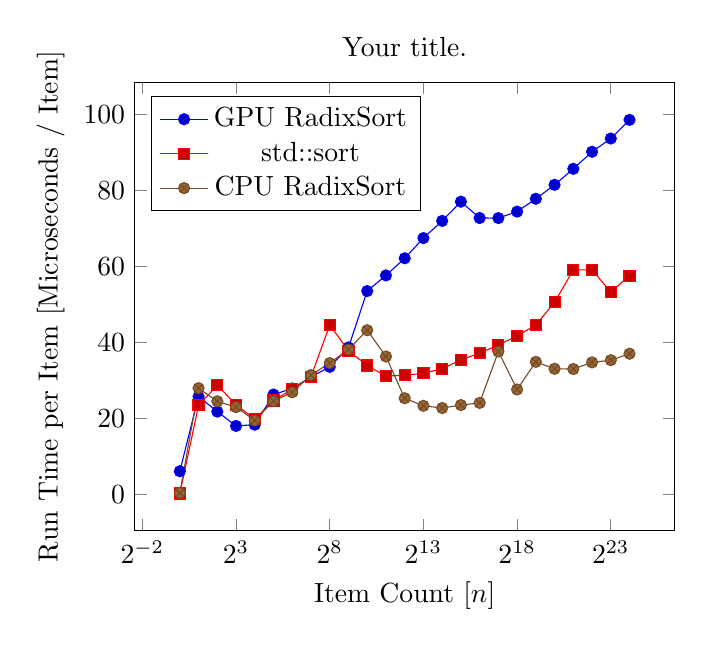
\begin{tikzpicture}[scale=1]
  \begin{axis}[
    title={Your title.},
    xlabel={Item Count [$n$]},
    ylabel={Run Time per Item [Microseconds / Item]},
    legend pos=north west,
    xmode=log,
    log basis x={2},
    ] 
    %% MULTIPLOT(threads) SELECT n AS x, (avg("wall-time") * 1.0 / n) AS y, MULTIPLOT
    %% FROM stats
    %% WHERE it > 0 AND "input-type"='uniform'
    %% GROUP BY MULTIPLOT,x ORDER BY MULTIPLOT,x
    \addplot coordinates { (1,6.14588) (2,25.8) (4,21.85) (8,18.075) (16,18.4125) (32,26.3438) (64,27.9469) (128,30.9563) (256,33.6352) (512,38.7367) (1024,53.5891) (2048,57.7013) (4096,62.2103) (8192,67.5351) (16384,72.0565) (32768,77.1085) (65536,72.8129) (131072,72.7906) (262144,74.5003) (524288,77.8793) (1048576,81.5511) (2097152,85.7657) (4194304,90.2553) (8388608,93.7425) (16777216,98.6555) };
    \addlegendentry{GPU RadixSort};
    \addplot coordinates { (1,0.2998) (2,23.5) (4,28.8) (8,23.675) (16,19.85) (32,24.75) (64,27.7625) (128,31.0453) (256,44.6383) (512,37.8852) (1024,33.967) (2048,31.1891) (4096,31.4354) (8192,31.9057) (16384,33.1395) (32768,35.4618) (65536,37.2686) (131072,39.349) (262144,41.8065) (524288,44.6163) (1048576,50.6581) (2097152,59.1302) (4194304,59.1624) (8388608,53.3066) (16777216,57.644) };
    \addlegendentry{std::sort};
    \addplot coordinates { (1,0.4005) (2,28) (4,24.55) (8,23.025) (16,19.525) (32,24.5875) (64,26.925) (128,31.4609) (256,34.6203) (512,38.2023) (1024,43.274) (2048,36.3531) (4096,25.3622) (8192,23.3748) (16384,22.7897) (32768,23.568) (65536,24.1379) (131072,37.6677) (262144,27.6724) (524288,34.9413) (1048576,33.1177) (2097152,33.0524) (4194304,34.8011) (8388608,35.3875) (16777216,37.0874) };
    \addlegendentry{CPU RadixSort};
  \end{axis}
\end{tikzpicture}
\caption{Runtimes of \texttt{std::sort} with uniform input. Mean of \iterationcnt~iterations.}
\label{fi:runningtime:uniform}
\end{figure}

\begin{figure}[h!]
\centering
\pgfplotsset{compat=1.5}
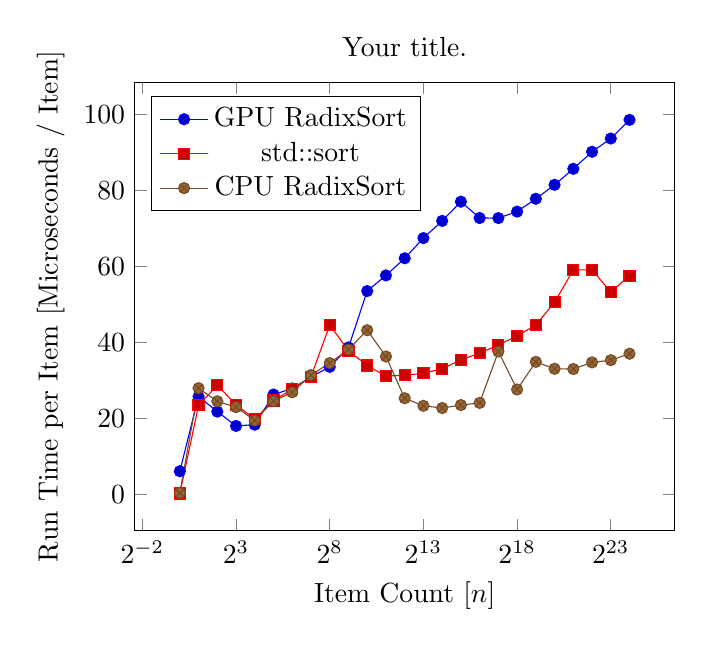
\begin{tikzpicture}[scale=1]
  \begin{axis}[
    title={Your title.},
    xlabel={Item Count [$n$]},
    ylabel={Run Time per Item [Microseconds / Item]},
    legend pos=north west,
    xmode=log,
    log basis x={2},
    ] 
    %% MULTIPLOT(threads) SELECT n AS x, (avg("wall-time") * 1.0 / n) AS y, MULTIPLOT
    %% FROM stats
    %% WHERE it > 0 AND "input-type"='uniform'
    %% GROUP BY MULTIPLOT,x ORDER BY MULTIPLOT,x
    \addplot coordinates { (1,6.14588) (2,25.8) (4,21.85) (8,18.075) (16,18.4125) (32,26.3438) (64,27.9469) (128,30.9563) (256,33.6352) (512,38.7367) (1024,53.5891) (2048,57.7013) (4096,62.2103) (8192,67.5351) (16384,72.0565) (32768,77.1085) (65536,72.8129) (131072,72.7906) (262144,74.5003) (524288,77.8793) (1048576,81.5511) (2097152,85.7657) (4194304,90.2553) (8388608,93.7425) (16777216,98.6555) };
    \addlegendentry{GPU RadixSort};
    \addplot coordinates { (1,0.2998) (2,23.5) (4,28.8) (8,23.675) (16,19.85) (32,24.75) (64,27.7625) (128,31.0453) (256,44.6383) (512,37.8852) (1024,33.967) (2048,31.1891) (4096,31.4354) (8192,31.9057) (16384,33.1395) (32768,35.4618) (65536,37.2686) (131072,39.349) (262144,41.8065) (524288,44.6163) (1048576,50.6581) (2097152,59.1302) (4194304,59.1624) (8388608,53.3066) (16777216,57.644) };
    \addlegendentry{std::sort};
    \addplot coordinates { (1,0.4005) (2,28) (4,24.55) (8,23.025) (16,19.525) (32,24.5875) (64,26.925) (128,31.4609) (256,34.6203) (512,38.2023) (1024,43.274) (2048,36.3531) (4096,25.3622) (8192,23.3748) (16384,22.7897) (32768,23.568) (65536,24.1379) (131072,37.6677) (262144,27.6724) (524288,34.9413) (1048576,33.1177) (2097152,33.0524) (4194304,34.8011) (8388608,35.3875) (16777216,37.0874) };
    \addlegendentry{CPU RadixSort};
  \end{axis}
\end{tikzpicture}
\caption{Runtimes of \texttt{std::sort} with uniform input. Mean of \iterationcnt~iterations.}
\label{fi:runningtime:uniform}
\end{figure}

\begin{figure}[h!]
\centering
\pgfplotsset{compat=1.5}
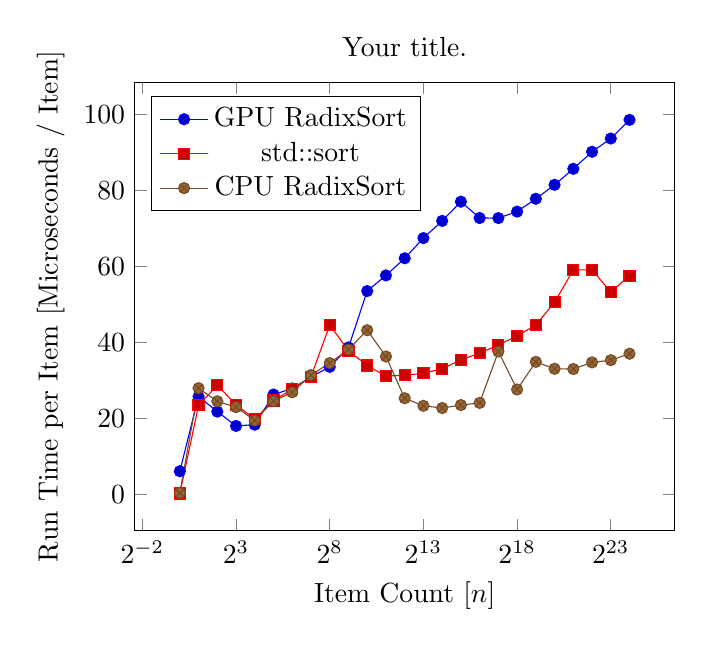
\begin{tikzpicture}[scale=1]
  \begin{axis}[
    title={Your title.},
    xlabel={Item Count [$n$]},
    ylabel={Run Time per Item [Microseconds / Item]},
    legend pos=north west,
    xmode=log,
    log basis x={2},
    ] 
    %% MULTIPLOT(threads) SELECT n AS x, (avg("wall-time") * 1.0 / n) AS y, MULTIPLOT
    %% FROM stats
    %% WHERE it > 0 AND "input-type"='uniform'
    %% GROUP BY MULTIPLOT,x ORDER BY MULTIPLOT,x
    \addplot coordinates { (1,6.14588) (2,25.8) (4,21.85) (8,18.075) (16,18.4125) (32,26.3438) (64,27.9469) (128,30.9563) (256,33.6352) (512,38.7367) (1024,53.5891) (2048,57.7013) (4096,62.2103) (8192,67.5351) (16384,72.0565) (32768,77.1085) (65536,72.8129) (131072,72.7906) (262144,74.5003) (524288,77.8793) (1048576,81.5511) (2097152,85.7657) (4194304,90.2553) (8388608,93.7425) (16777216,98.6555) };
    \addlegendentry{GPU RadixSort};
    \addplot coordinates { (1,0.2998) (2,23.5) (4,28.8) (8,23.675) (16,19.85) (32,24.75) (64,27.7625) (128,31.0453) (256,44.6383) (512,37.8852) (1024,33.967) (2048,31.1891) (4096,31.4354) (8192,31.9057) (16384,33.1395) (32768,35.4618) (65536,37.2686) (131072,39.349) (262144,41.8065) (524288,44.6163) (1048576,50.6581) (2097152,59.1302) (4194304,59.1624) (8388608,53.3066) (16777216,57.644) };
    \addlegendentry{std::sort};
    \addplot coordinates { (1,0.4005) (2,28) (4,24.55) (8,23.025) (16,19.525) (32,24.5875) (64,26.925) (128,31.4609) (256,34.6203) (512,38.2023) (1024,43.274) (2048,36.3531) (4096,25.3622) (8192,23.3748) (16384,22.7897) (32768,23.568) (65536,24.1379) (131072,37.6677) (262144,27.6724) (524288,34.9413) (1048576,33.1177) (2097152,33.0524) (4194304,34.8011) (8388608,35.3875) (16777216,37.0874) };
    \addlegendentry{CPU RadixSort};
  \end{axis}
\end{tikzpicture}
\caption{Running times of \texttt{std::sort} with uniform input. Mean of \iterationcnt~iterations.}
\label{fi:runningtime:uniform}
\end{figure}

\bibliographystyle{splncs03}
\bibliography{sources}

\end{document}
